\documentclass[11pt]{article}\usepackage[]{graphicx}\usepackage[]{color}
%% maxwidth is the original width if it is less than linewidth
%% otherwise use linewidth (to make sure the graphics do not exceed the margin)
\makeatletter
\def\maxwidth{ %
  \ifdim\Gin@nat@width>\linewidth
    \linewidth
  \else
    \Gin@nat@width
  \fi
}
\makeatother

\definecolor{fgcolor}{rgb}{0.345, 0.345, 0.345}
\newcommand{\hlnum}[1]{\textcolor[rgb]{0.686,0.059,0.569}{#1}}%
\newcommand{\hlstr}[1]{\textcolor[rgb]{0.192,0.494,0.8}{#1}}%
\newcommand{\hlcom}[1]{\textcolor[rgb]{0.678,0.584,0.686}{\textit{#1}}}%
\newcommand{\hlopt}[1]{\textcolor[rgb]{0,0,0}{#1}}%
\newcommand{\hlstd}[1]{\textcolor[rgb]{0.345,0.345,0.345}{#1}}%
\newcommand{\hlkwa}[1]{\textcolor[rgb]{0.161,0.373,0.58}{\textbf{#1}}}%
\newcommand{\hlkwb}[1]{\textcolor[rgb]{0.69,0.353,0.396}{#1}}%
\newcommand{\hlkwc}[1]{\textcolor[rgb]{0.333,0.667,0.333}{#1}}%
\newcommand{\hlkwd}[1]{\textcolor[rgb]{0.737,0.353,0.396}{\textbf{#1}}}%

\usepackage{framed}
\makeatletter
\newenvironment{kframe}{%
 \def\at@end@of@kframe{}%
 \ifinner\ifhmode%
  \def\at@end@of@kframe{\end{minipage}}%
  \begin{minipage}{\columnwidth}%
 \fi\fi%
 \def\FrameCommand##1{\hskip\@totalleftmargin \hskip-\fboxsep
 \colorbox{shadecolor}{##1}\hskip-\fboxsep
     % There is no \\@totalrightmargin, so:
     \hskip-\linewidth \hskip-\@totalleftmargin \hskip\columnwidth}%
 \MakeFramed {\advance\hsize-\width
   \@totalleftmargin\z@ \linewidth\hsize
   \@setminipage}}%
 {\par\unskip\endMakeFramed%
 \at@end@of@kframe}
\makeatother

\definecolor{shadecolor}{rgb}{.97, .97, .97}
\definecolor{messagecolor}{rgb}{0, 0, 0}
\definecolor{warningcolor}{rgb}{1, 0, 1}
\definecolor{errorcolor}{rgb}{1, 0, 0}
\newenvironment{knitrout}{}{} % an empty environment to be redefined in TeX

\usepackage{alltt}
\usepackage{amsmath}
\usepackage{listings}
\usepackage{stmaryrd}
\usepackage{bbm}
\usepackage{amsmath}
\usepackage{mathtools}
\usepackage{pdfpages}
\usepackage{breqn}



\newcount\colveccount
\newcommand*\colvec[1]{
        \global\colveccount#1
        \begin{pmatrix}
        \colvecnext
}
\def\colvecnext#1{
        #1
        \global\advance\colveccount-1
        \ifnum\colveccount>0
                \\
                \expandafter\colvecnext
        \else
                \end{pmatrix}
        \fi
}
\newcommand{\argmin}{\arg\!\min}

\author{Thibault Doutre, Student ID 26980469}
\title{STAT230 HW 8 \\
University of California, Berkeley}
\date{\today}
\IfFileExists{upquote.sty}{\usepackage{upquote}}{}
\begin{document}

\maketitle
\section{PART 1}
\begin{knitrout}
\definecolor{shadecolor}{rgb}{0.969, 0.969, 0.969}\color{fgcolor}\begin{kframe}
\begin{alltt}
\hlstd{xUnique} \hlkwb{=} \hlnum{1}\hlopt{:}\hlnum{5}
\hlstd{trueCoeff} \hlkwb{=} \hlkwd{c}\hlstd{(}\hlnum{0}\hlstd{,} \hlnum{1}\hlstd{,} \hlnum{1}\hlstd{)}

\hlstd{genData} \hlkwb{=} \hlkwa{function}\hlstd{(}\hlkwc{coefs} \hlstd{=} \hlkwd{c}\hlstd{(}\hlnum{0}\hlstd{,} \hlnum{1}\hlstd{,} \hlnum{1}\hlstd{),} \hlkwc{xs} \hlstd{=} \hlnum{1}\hlopt{:}\hlnum{5}\hlstd{,} \hlkwc{dupl} \hlstd{=} \hlnum{10}\hlstd{,}
                   \hlkwc{sd} \hlstd{=} \hlnum{5}\hlstd{,} \hlkwc{seed}\hlstd{=}\hlnum{2222}\hlstd{)\{}
  \hlcom{### This function creates the artificial data}
  \hlkwd{set.seed}\hlstd{(seed)}
  \hlstd{x} \hlkwb{=} \hlkwd{rep}\hlstd{(xs,} \hlkwc{each} \hlstd{= dupl)}
  \hlstd{y} \hlkwb{=} \hlstd{coefs[}\hlnum{1}\hlstd{]} \hlopt{+} \hlstd{coefs[}\hlnum{2}\hlstd{]}\hlopt{*}\hlstd{x} \hlopt{+} \hlstd{coefs[}\hlnum{3}\hlstd{]} \hlopt{*} \hlstd{x}\hlopt{^}\hlnum{2} \hlopt{+}
    \hlkwd{rnorm}\hlstd{(}\hlkwd{length}\hlstd{(x),} \hlnum{0}\hlstd{, sd)}
  \hlkwd{return}\hlstd{(}\hlkwd{data.frame}\hlstd{(x, y))}
\hlstd{\}}

\hlstd{data} \hlkwb{=} \hlkwd{genData}\hlstd{()}

\hlcom{## # Part 1}

\hlstd{genBootY} \hlkwb{=} \hlkwa{function}\hlstd{(}\hlkwc{x}\hlstd{,} \hlkwc{y}\hlstd{,} \hlkwc{rep} \hlstd{=} \hlnum{TRUE}\hlstd{)\{}
  \hlcom{### For each unique x value, take a sample of the}
  \hlcom{### corresponding y values, with or without replacement.}
  \hlcom{### Return a vector of random y values the same length as y}
  \hlcom{### You can assume that the xs are sorted}
  \hlstd{res} \hlkwb{=} \hlstd{x}
  \hlkwa{for} \hlstd{(xi} \hlkwa{in} \hlkwd{unique}\hlstd{(x))\{}
    \hlstd{y_values} \hlkwb{=} \hlstd{y[x} \hlopt{==} \hlstd{xi]}
    \hlstd{y_sample} \hlkwb{=} \hlkwd{sample}\hlstd{(y_values,} \hlnum{10}\hlstd{,} \hlkwc{replace} \hlstd{= rep)}
    \hlstd{res[x} \hlopt{==} \hlstd{xi]} \hlkwb{=} \hlstd{y_sample}
  \hlstd{\}}
  \hlstd{res}
\hlstd{\}}

\hlstd{genBootR} \hlkwb{=} \hlkwa{function}\hlstd{(}\hlkwc{fit}\hlstd{,} \hlkwc{err}\hlstd{,} \hlkwc{rep} \hlstd{=} \hlnum{TRUE}\hlstd{)\{}
  \hlcom{### Sample the errors }
  \hlcom{### Add the errors to the fit to create a y vector}
  \hlcom{### Return a vector of y values the same length as fit}
  \hlstd{err_boot} \hlkwb{=} \hlkwd{sample}\hlstd{(err,} \hlkwd{length}\hlstd{(err),} \hlkwc{replace} \hlstd{= rep)}
  \hlstd{y} \hlkwb{=} \hlstd{fit} \hlopt{+} \hlstd{err_boot}
  \hlstd{y}

\hlstd{\}}
\end{alltt}
\end{kframe}
\end{knitrout}

\section{PART 2}
\begin{knitrout}
\definecolor{shadecolor}{rgb}{0.969, 0.969, 0.969}\color{fgcolor}\begin{kframe}
\begin{alltt}
\hlcom{## # Part 2}

\hlstd{fitModel} \hlkwb{=} \hlkwa{function}\hlstd{(}\hlkwc{x}\hlstd{,} \hlkwc{y}\hlstd{,} \hlkwc{degree} \hlstd{=} \hlnum{1}\hlstd{)\{}
  \hlcom{### use the lm function to fit a line of a quadratic }
  \hlcom{### e.g. y ~ x or y ~ x + I(x^2)}
  \hlcom{### y and x are numeric vectors of the same length}
  \hlcom{### Return the coefficients as a vector }
  \hlkwa{if} \hlstd{(degree} \hlopt{==} \hlnum{1}\hlstd{)\{}
    \hlstd{lm.fit} \hlkwb{=} \hlkwd{lm}\hlstd{(y} \hlopt{~} \hlstd{x)}
  \hlstd{\}}
  \hlkwa{if} \hlstd{(degree} \hlopt{==} \hlnum{2}\hlstd{)\{}
    \hlstd{lm.fit} \hlkwb{=} \hlkwd{lm}\hlstd{(y} \hlopt{~} \hlstd{x} \hlopt{+} \hlkwd{I}\hlstd{(x}\hlopt{^}\hlnum{2}\hlstd{))}
  \hlstd{\}}
  \hlkwd{as.vector}\hlstd{(lm.fit}\hlopt{$}\hlstd{coefficients)}
\hlstd{\}}
\end{alltt}
\end{kframe}
\end{knitrout}

\section{PART 3}
\begin{knitrout}
\definecolor{shadecolor}{rgb}{0.969, 0.969, 0.969}\color{fgcolor}\begin{kframe}
\begin{alltt}
\hlcom{## # Part 3}

\hlstd{oneBoot} \hlkwb{=} \hlkwa{function}\hlstd{(}\hlkwc{data}\hlstd{,} \hlkwc{err1}\hlstd{,} \hlkwc{err2}\hlstd{)\{}
  \hlcom{### data are your data (from call to getData)}
  \hlcom{###  err1 are errors from fit of line to data}
  \hlcom{###  err2 are errors from fit of quadratic to data}
  \hlcom{###  generate three bootstrap samples }
  \hlcom{###  A. use genBootY}
  \hlcom{###  B. use genBootR and errors from linear fit}
  \hlcom{###  C. use genBootR and errors from quadratic fit}
  \hlstd{y_A} \hlkwb{=} \hlkwd{genBootY}\hlstd{(data}\hlopt{$}\hlstd{x, data}\hlopt{$}\hlstd{y,} \hlkwc{rep} \hlstd{=} \hlnum{TRUE}\hlstd{)}
  \hlstd{y_B} \hlkwb{=} \hlkwd{genBootR}\hlstd{(data}\hlopt{$}\hlstd{y, err1,} \hlkwc{rep} \hlstd{=} \hlnum{FALSE}\hlstd{)}
  \hlstd{y_C} \hlkwb{=} \hlkwd{genBootR}\hlstd{(data}\hlopt{$}\hlstd{y, err2,} \hlkwc{rep} \hlstd{=} \hlnum{FALSE}\hlstd{)}

  \hlcom{### For A, fit a line to data$x and new y's}
  \hlcom{### Repeat to fit a quadratic}
  \hlcom{### For B, fit a line to data$x and the new y's}
  \hlcom{### For C, fit a quadratic to data$x and new y's}
  \hlstd{fit.A1} \hlkwb{=} \hlkwd{fitModel}\hlstd{(data}\hlopt{$}\hlstd{x, y_A,} \hlkwc{degree} \hlstd{=} \hlnum{1}\hlstd{)}
  \hlstd{fit.A2} \hlkwb{=} \hlkwd{fitModel}\hlstd{(data}\hlopt{$}\hlstd{x, y_A,} \hlkwc{degree} \hlstd{=} \hlnum{2}\hlstd{)}
  \hlstd{fit.B1} \hlkwb{=} \hlkwd{fitModel}\hlstd{(data}\hlopt{$}\hlstd{x, y_B,} \hlkwc{degree} \hlstd{=} \hlnum{1}\hlstd{)}
  \hlstd{fit.C2} \hlkwb{=} \hlkwd{fitModel}\hlstd{(data}\hlopt{$}\hlstd{x, y_C,} \hlkwc{degree} \hlstd{=} \hlnum{2}\hlstd{)}

  \hlcom{### Return the coefficients from the 4 fits in a list }
  \hlkwd{list}\hlstd{(}\hlkwc{A1} \hlstd{= fit.A1,} \hlkwc{A2} \hlstd{= fit.A2,} \hlkwc{B1} \hlstd{= fit.B1,} \hlkwc{C2} \hlstd{= fit.C2)}
\hlstd{\}}
\end{alltt}
\end{kframe}
\end{knitrout}

\section{PART 4}
\begin{knitrout}
\definecolor{shadecolor}{rgb}{0.969, 0.969, 0.969}\color{fgcolor}\begin{kframe}
\begin{alltt}
\hlstd{repBoot} \hlkwb{=} \hlkwa{function}\hlstd{(}\hlkwc{data}\hlstd{,} \hlkwc{B} \hlstd{=} \hlnum{1000}\hlstd{)\{}

  \hlcom{### replicate a call to oneBoot B times}
  \hlcom{### format the return value so that you have a list of}
  \hlcom{### length 4, one for each set of coefficients}
  \hlcom{### each element will contain a data frame with B rows}
  \hlcom{### and two or three columns, depending on whether the }
  \hlcom{### fit is for a line or a quadratic}
  \hlcom{### Return this list}
  \hlstd{res.A1} \hlkwb{=} \hlkwd{as.data.frame}\hlstd{(}\hlkwd{matrix}\hlstd{(}\hlnum{NA}\hlstd{,} \hlkwc{nrow} \hlstd{= B,} \hlkwc{ncol} \hlstd{=} \hlnum{2}\hlstd{))}
  \hlstd{res.A2} \hlkwb{=} \hlkwd{as.data.frame}\hlstd{(}\hlkwd{matrix}\hlstd{(}\hlnum{NA}\hlstd{,} \hlkwc{nrow} \hlstd{= B,} \hlkwc{ncol} \hlstd{=} \hlnum{3}\hlstd{))}
  \hlstd{res.B1} \hlkwb{=} \hlkwd{as.data.frame}\hlstd{(}\hlkwd{matrix}\hlstd{(}\hlnum{NA}\hlstd{,} \hlkwc{nrow} \hlstd{= B,} \hlkwc{ncol} \hlstd{=} \hlnum{2}\hlstd{))}
  \hlstd{res.C2} \hlkwb{=} \hlkwd{as.data.frame}\hlstd{(}\hlkwd{matrix}\hlstd{(}\hlnum{NA}\hlstd{,} \hlkwc{nrow} \hlstd{= B,} \hlkwc{ncol} \hlstd{=} \hlnum{3}\hlstd{))}

  \hlstd{err1} \hlkwb{=} \hlkwd{rnorm}\hlstd{(}\hlkwd{nrow}\hlstd{(data))}
  \hlstd{err2} \hlkwb{=} \hlkwd{rnorm}\hlstd{(}\hlkwd{nrow}\hlstd{(data))}

  \hlkwa{for} \hlstd{(i} \hlkwa{in} \hlnum{1}\hlopt{:}\hlstd{B)\{}
    \hlstd{res} \hlkwb{=} \hlkwd{oneBoot}\hlstd{(data, err1, err2)}
    \hlstd{res.A1[i,]} \hlkwb{=} \hlstd{res}\hlopt{$}\hlstd{A1}
    \hlstd{res.A2[i,]} \hlkwb{=} \hlstd{res}\hlopt{$}\hlstd{A2}
    \hlstd{res.B1[i,]} \hlkwb{=} \hlstd{res}\hlopt{$}\hlstd{B1}
    \hlstd{res.C2[i,]} \hlkwb{=} \hlstd{res}\hlopt{$}\hlstd{C2}
  \hlstd{\}}

  \hlkwd{list}\hlstd{(}\hlkwc{A1} \hlstd{= res.A1,} \hlkwc{A2} \hlstd{= res.A2,} \hlkwc{B1} \hlstd{= res.B1,} \hlkwc{C2} \hlstd{= res.C2)}

\hlstd{\}}

\hlstd{repBootConf} \hlkwb{=} \hlkwa{function}\hlstd{(}\hlkwc{data}\hlstd{,} \hlkwc{B} \hlstd{=} \hlnum{1000}\hlstd{)\{}
  \hlcom{### For each of the four variations, return a bootstrap }
  \hlcom{### 95% confidence interval for the linear coefficient }
  \hlcom{### for x.}
  \hlstd{res} \hlkwb{=} \hlkwd{repBoot}\hlstd{(data)}
  \hlstd{conf.A1} \hlkwb{=} \hlkwd{as.vector}\hlstd{(}\hlkwd{t.test}\hlstd{(res}\hlopt{$}\hlstd{A1[,}\hlnum{2}\hlstd{])}\hlopt{$}\hlstd{conf.int[}\hlnum{1}\hlopt{:}\hlnum{2}\hlstd{])}
  \hlstd{conf.A2} \hlkwb{=} \hlkwd{as.vector}\hlstd{(}\hlkwd{t.test}\hlstd{(res}\hlopt{$}\hlstd{A2[,}\hlnum{2}\hlstd{])}\hlopt{$}\hlstd{conf.int[}\hlnum{1}\hlopt{:}\hlnum{2}\hlstd{])}
  \hlstd{conf.B1} \hlkwb{=} \hlkwd{as.vector}\hlstd{(}\hlkwd{t.test}\hlstd{(res}\hlopt{$}\hlstd{B1[,}\hlnum{2}\hlstd{])}\hlopt{$}\hlstd{conf.int[}\hlnum{1}\hlopt{:}\hlnum{2}\hlstd{])}
  \hlstd{conf.C2} \hlkwb{=} \hlkwd{as.vector}\hlstd{(}\hlkwd{t.test}\hlstd{(res}\hlopt{$}\hlstd{C2[,}\hlnum{2}\hlstd{])}\hlopt{$}\hlstd{conf.int[}\hlnum{1}\hlopt{:}\hlnum{2}\hlstd{])}

  \hlkwd{list}\hlstd{(}\hlkwc{A1} \hlstd{= conf.A1,} \hlkwc{A2} \hlstd{= conf.A2,} \hlkwc{B1} \hlstd{= conf.B1,} \hlkwc{C2} \hlstd{= conf.C2)}
\hlstd{\}}
\end{alltt}
\end{kframe}
\end{knitrout}

\section{PART 5}
\begin{knitrout}
\definecolor{shadecolor}{rgb}{0.969, 0.969, 0.969}\color{fgcolor}\begin{kframe}
\begin{alltt}
\hlcom{## # Part 5}

\hlstd{bootPlot} \hlkwb{=} \hlkwa{function}\hlstd{(}\hlkwc{data}\hlstd{,} \hlkwc{coeff}\hlstd{,} \hlkwc{trueCoeff}\hlstd{)\{}
  \hlcom{### data is the original data set}
  \hlcom{### coeff is a data frame from repBoot}
  \hlcom{### trueCoeff contains the true coefficients that generated}
  \hlcom{### data}

  \hlcom{### Make a scatter plot of data}
  \hlcom{### Use mapply to add lines or curves for each row in coeff}
  \hlcom{### Use transparency}
  \hlcom{### Use trueCoeff to add line or curve - make it stand out}

  \hlstd{draw_line} \hlkwb{=} \hlkwa{function}\hlstd{(}\hlkwc{row}\hlstd{,} \hlkwc{lwd} \hlstd{=} \hlnum{.03}\hlstd{,} \hlkwc{col} \hlstd{=} \hlstr{"darkgray"}\hlstd{)\{}
    \hlkwa{if} \hlstd{(}\hlkwd{length}\hlstd{(row)} \hlopt{==} \hlnum{2}\hlstd{)\{}
      \hlkwd{abline}\hlstd{(}\hlkwd{as.numeric}\hlstd{(row[}\hlnum{1}\hlstd{]),} \hlkwd{as.numeric}\hlstd{(row[}\hlnum{2}\hlstd{]),}  \hlkwc{lwd} \hlstd{= lwd,} \hlkwc{col} \hlstd{= col)}
    \hlstd{\}}
    \hlkwa{if} \hlstd{(}\hlkwd{length}\hlstd{(row)} \hlopt{==} \hlnum{3}\hlstd{)\{}
      \hlstd{x} \hlkwb{=} \hlkwd{seq}\hlstd{(}\hlnum{1}\hlstd{,}\hlnum{5}\hlstd{,}\hlkwc{by}\hlstd{=}\hlnum{0.1}\hlstd{)}
      \hlstd{y} \hlkwb{=} \hlkwd{as.numeric}\hlstd{(row[}\hlnum{1}\hlstd{])} \hlopt{+} \hlkwd{as.numeric}\hlstd{(row[}\hlnum{2}\hlstd{])}\hlopt{*}\hlstd{x} \hlopt{+} \hlkwd{as.numeric}\hlstd{(row[}\hlnum{3}\hlstd{])}\hlopt{*}\hlstd{(x}\hlopt{^}\hlnum{2}\hlstd{)}
      \hlkwd{lines}\hlstd{(x, y,} \hlkwc{lwd} \hlstd{= lwd,} \hlkwc{col} \hlstd{= col)}
    \hlstd{\}}
  \hlstd{\}}

  \hlstd{plot_model} \hlkwb{=} \hlkwa{function}\hlstd{(}\hlkwc{coeff_values}\hlstd{)\{}
    \hlkwd{plot}\hlstd{(data)}
    \hlkwd{apply}\hlstd{(coeff_values,} \hlnum{1}\hlstd{, draw_line)}
    \hlstd{x} \hlkwb{=} \hlkwd{seq}\hlstd{(}\hlnum{1}\hlstd{,}\hlnum{5}\hlstd{,}\hlkwc{by}\hlstd{=}\hlnum{0.1}\hlstd{)}
    \hlstd{y} \hlkwb{=} \hlkwd{as.numeric}\hlstd{(trueCoeff[}\hlnum{1}\hlstd{])} \hlopt{+}
      \hlkwd{as.numeric}\hlstd{(trueCoeff[}\hlnum{2}\hlstd{])}\hlopt{*}\hlstd{x} \hlopt{+}
      \hlkwd{as.numeric}\hlstd{(trueCoeff[}\hlnum{3}\hlstd{])}\hlopt{*}\hlstd{(x}\hlopt{^}\hlnum{2}\hlstd{)}
    \hlkwd{lines}\hlstd{(x, y,} \hlkwc{lwd} \hlstd{=} \hlnum{4}\hlstd{,} \hlkwc{col} \hlstd{=} \hlstr{"black"}\hlstd{,} \hlkwc{lty}\hlstd{=}\hlnum{2}\hlstd{)}
  \hlstd{\}}

  \hlkwd{plot_model}\hlstd{(coeff)}
\hlstd{\}}

\hlcom{### Run your simulation}

\hlstd{xUnique} \hlkwb{=} \hlnum{1}\hlopt{:}\hlnum{5}
\hlstd{trueCoeff} \hlkwb{=} \hlkwd{c}\hlstd{(}\hlnum{0}\hlstd{,} \hlnum{1}\hlstd{,} \hlnum{1}\hlstd{)}
\hlstd{myData} \hlkwb{=} \hlkwd{genData}\hlstd{(}\hlkwc{coefs} \hlstd{= trueCoeff,} \hlkwc{xs} \hlstd{= xUnique)}
\hlstd{expt} \hlkwb{=} \hlkwd{repBoot}\hlstd{(}\hlkwc{data} \hlstd{= myData )}
\hlkwd{par}\hlstd{(}\hlkwc{mfrow} \hlstd{=} \hlkwd{c}\hlstd{(}\hlnum{2}\hlstd{,} \hlnum{2}\hlstd{))}
\hlkwd{bootPlot}\hlstd{(}\hlkwc{data} \hlstd{= myData,} \hlkwc{coeff} \hlstd{= expt[[}\hlnum{1}\hlstd{]], trueCoeff)}
\hlkwd{title}\hlstd{(}\hlstr{"A1"}\hlstd{)}
\hlkwd{bootPlot}\hlstd{(}\hlkwc{data} \hlstd{= myData,} \hlkwc{coeff} \hlstd{= expt[[}\hlnum{2}\hlstd{]], trueCoeff)}
\hlkwd{title}\hlstd{(}\hlstr{"A2"}\hlstd{)}
\hlkwd{bootPlot}\hlstd{(}\hlkwc{data} \hlstd{= myData,} \hlkwc{coeff} \hlstd{= expt[[}\hlnum{3}\hlstd{]], trueCoeff)}
\hlkwd{title}\hlstd{(}\hlstr{"B1"}\hlstd{)}
\hlkwd{bootPlot}\hlstd{(}\hlkwc{data} \hlstd{= myData,} \hlkwc{coeff} \hlstd{= expt[[}\hlnum{4}\hlstd{]], trueCoeff)}
\hlkwd{title}\hlstd{(}\hlstr{"C2"}\hlstd{)}
\end{alltt}
\end{kframe}
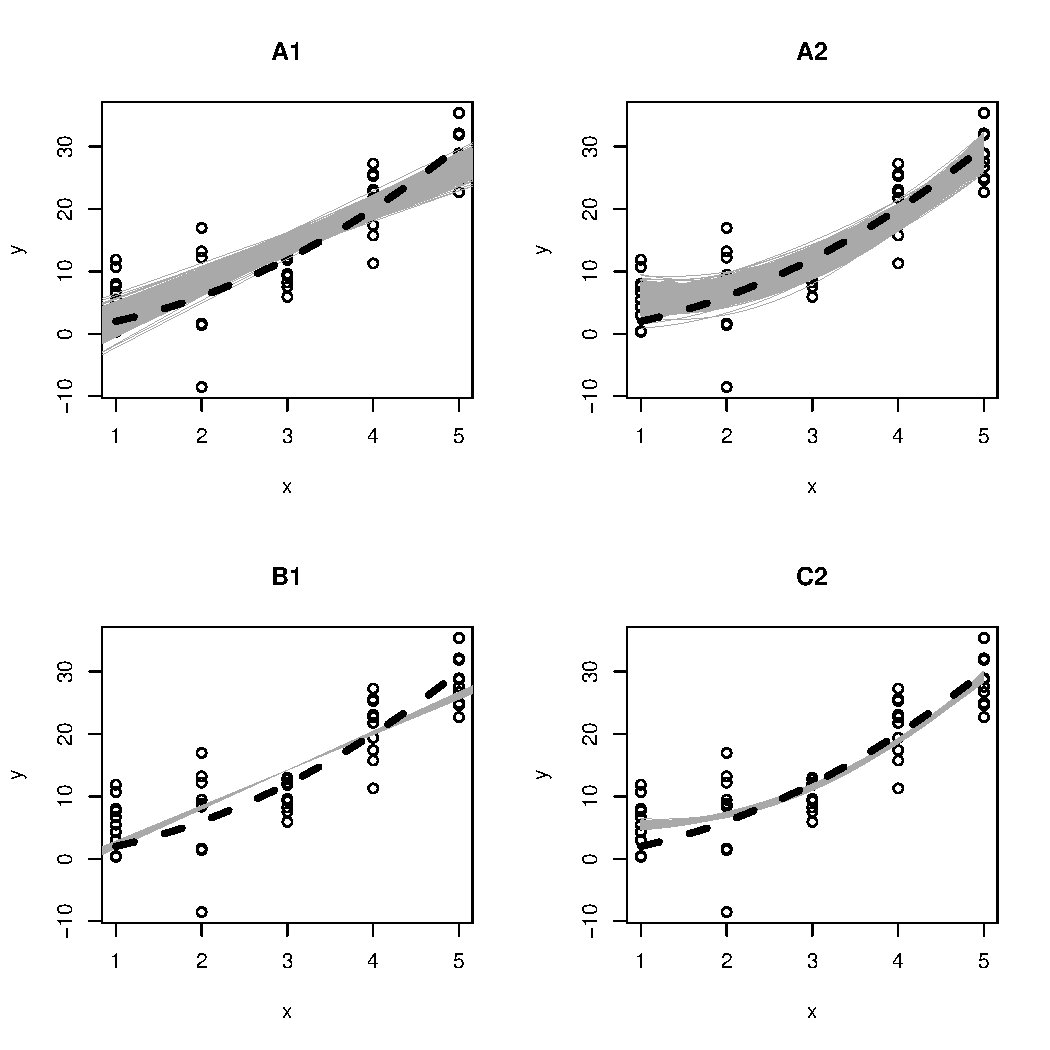
\includegraphics[width=\maxwidth]{figure/unnamed-chunk-6-1} 
\begin{kframe}\begin{alltt}
\hlkwd{par}\hlstd{(}\hlkwc{mfrow} \hlstd{=} \hlkwd{c}\hlstd{(}\hlnum{1}\hlstd{,} \hlnum{1}\hlstd{))}
\end{alltt}
\end{kframe}
\end{knitrout}
\begin{itemize}
\item When is the variability smallest?\\
With the second method
\item Is there a problem with bias when the model being fitted is wrong?\\ 
No bias when the model being fitted is linear
\item Is there a problem with basing the bootstrap on the data, i.e. are the data close to the truth? \\
Data seem close to the truth, except for points with low x values
\item Are any problems you find worse for one method than the other?\\
First method leads to less variability, but depends on the choice of the errors. Also we may need to jitter the data along the x axis.
\end{itemize}

\section{PART 6}
\begin{knitrout}
\definecolor{shadecolor}{rgb}{0.969, 0.969, 0.969}\color{fgcolor}\begin{kframe}
\begin{alltt}
\hlcom{### PART 6.}
\hlcom{### Generate data}
\hlkwd{set.seed}\hlstd{(}\hlnum{1}\hlstd{)}
\hlstd{W} \hlkwb{=} \hlkwd{rnorm}\hlstd{(}\hlnum{100}\hlstd{,}\hlnum{1}\hlopt{:}\hlnum{100}\hlopt{/}\hlnum{5}\hlstd{)}

\hlcom{# Parameters to be estimated}
\hlstd{a} \hlkwb{=} \hlkwd{c}\hlstd{(}\hlnum{1}\hlstd{,}\hlnum{2}\hlstd{)}
\hlstd{b} \hlkwb{=} \hlnum{0.3}
\hlstd{c} \hlkwb{=} \hlnum{4}
\hlstd{beta} \hlkwb{=} \hlkwd{c}\hlstd{(a[}\hlnum{1}\hlstd{],a[}\hlnum{2}\hlstd{],b,c)}

\hlcom{# Covariance matrix of the errors}
\hlstd{K} \hlkwb{=} \hlkwd{matrix}\hlstd{(}\hlkwd{c}\hlstd{(}\hlnum{1}\hlstd{,}\hlnum{0.5}\hlstd{,}\hlnum{0.5}\hlstd{,}\hlnum{2}\hlstd{),}\hlkwc{ncol}\hlstd{=}\hlnum{2}\hlstd{)}

\hlcom{# Generate errors function}
\hlstd{generate_errors} \hlkwb{=} \hlkwa{function}\hlstd{(}\hlkwc{n} \hlstd{=} \hlnum{50}\hlstd{)\{}
  \hlcom{# Define parameters}
  \hlstd{rho} \hlkwb{=} \hlnum{0.5}\hlopt{/}\hlkwd{sqrt}\hlstd{(}\hlnum{2}\hlstd{)}
  \hlstd{mu1}\hlkwb{=}\hlnum{0}\hlstd{; s1}\hlkwb{=}\hlnum{1}\hlstd{; mu2}\hlkwb{=}\hlnum{0}\hlstd{; s2}\hlkwb{=}\hlkwd{sqrt}\hlstd{(}\hlnum{2}\hlstd{)}

  \hlcom{# Define X, Y and Z with the bivariate normal relationship}
  \hlstd{X} \hlkwb{=} \hlkwd{rnorm}\hlstd{(n)}
  \hlstd{Z} \hlkwb{=} \hlkwd{rnorm}\hlstd{(n)}
  \hlstd{eps} \hlkwb{=} \hlkwd{sqrt}\hlstd{(}\hlnum{1}\hlopt{-}\hlstd{rho}\hlopt{^}\hlnum{2}\hlstd{)} \hlopt{*} \hlstd{Z}
  \hlstd{Y} \hlkwb{=} \hlstd{rho} \hlopt{*} \hlstd{X} \hlopt{+} \hlstd{eps}

  \hlcom{# Adjust means and variances}
  \hlstd{Y} \hlkwb{=} \hlstd{(Y}\hlopt{-}\hlkwd{mean}\hlstd{(Y))}\hlopt{/}\hlkwd{sd}\hlstd{(Y)}\hlopt{*}\hlstd{s2}\hlopt{+}\hlstd{mu2}
  \hlstd{X} \hlkwb{=} \hlstd{(X}\hlopt{-}\hlkwd{mean}\hlstd{(X))}\hlopt{/}\hlkwd{sd}\hlstd{(X)}\hlopt{*}\hlstd{s1}\hlopt{+}\hlstd{mu1}

  \hlcom{# Adjust rho by transforming Y}
  \hlstd{rho_hat} \hlkwb{=} \hlkwd{cor}\hlstd{(X,Y)}
  \hlstd{a} \hlkwb{=} \hlstd{s1}\hlopt{^}\hlnum{4}\hlopt{*}\hlstd{(rho}\hlopt{^}\hlnum{2}\hlopt{-}\hlnum{1}\hlstd{)}
  \hlstd{b} \hlkwb{=} \hlnum{2}\hlopt{*}\hlstd{rho_hat}\hlopt{*}\hlstd{s1}\hlopt{^}\hlnum{3}\hlopt{*}\hlstd{s2}\hlopt{*}\hlstd{(rho}\hlopt{^}\hlnum{2}\hlopt{-}\hlnum{1}\hlstd{)}
  \hlstd{c} \hlkwb{=} \hlstd{(rho}\hlopt{^}\hlnum{2}\hlopt{-}\hlstd{rho_hat}\hlopt{^}\hlnum{2}\hlstd{)}\hlopt{*}\hlstd{s2}\hlopt{^}\hlnum{2}\hlopt{*}\hlstd{s1}\hlopt{^}\hlnum{2}
  \hlstd{delta} \hlkwb{=} \hlstd{b}\hlopt{^}\hlnum{2}\hlopt{-}\hlnum{4}\hlopt{*}\hlstd{a}\hlopt{*}\hlstd{c}
  \hlstd{correction} \hlkwb{=} \hlstd{(}\hlopt{-}\hlstd{b}\hlopt{-}\hlkwd{sqrt}\hlstd{(delta))}\hlopt{/}\hlstd{(}\hlnum{2}\hlopt{*}\hlstd{a)}
  \hlstd{Y}\hlkwb{=}\hlstd{Y}\hlopt{+}\hlstd{correction}\hlopt{*}\hlstd{X}

  \hlcom{# Adjust means and variances}
  \hlstd{Y} \hlkwb{=} \hlstd{(Y}\hlopt{-}\hlkwd{mean}\hlstd{(Y))}\hlopt{/}\hlkwd{sd}\hlstd{(Y)}\hlopt{*}\hlstd{s2}\hlopt{+}\hlstd{mu2}
  \hlstd{X} \hlkwb{=} \hlstd{(X}\hlopt{-}\hlkwd{mean}\hlstd{(X))}\hlopt{/}\hlkwd{sd}\hlstd{(X)}\hlopt{*}\hlstd{s1}\hlopt{+}\hlstd{mu1}

  \hlkwd{return}\hlstd{(}\hlkwd{cbind}\hlstd{(X,Y))}
\hlstd{\}}

\hlcom{# Generate errors}
\hlstd{epsilons} \hlkwb{=} \hlkwd{generate_errors}\hlstd{()}
\hlkwd{cov}\hlstd{(epsilons)}
\end{alltt}
\begin{lstlisting}[basicstyle=\ttfamily,breaklines=true]
##     X   Y
## X 1.0 0.5
## Y 0.5 2.0
\end{lstlisting}
\begin{alltt}
\hlcom{# Generate Y}
\hlstd{Y} \hlkwb{=} \hlkwd{c}\hlstd{(}\hlnum{0}\hlstd{,}\hlnum{0}\hlstd{,W)}
\hlstd{m} \hlkwb{=} \hlnum{50}
\hlkwa{for} \hlstd{(t} \hlkwa{in} \hlnum{1}\hlopt{:}\hlnum{50}\hlstd{) \{}
  \hlkwa{for} \hlstd{(j} \hlkwa{in} \hlnum{1}\hlopt{:}\hlnum{2}\hlstd{)\{}
    \hlcom{# Y_tj}
    \hlstd{Y[}\hlnum{2}\hlopt{*}\hlstd{t}\hlopt{+}\hlstd{j]} \hlkwb{=} \hlstd{a[j]} \hlopt{+} \hlstd{b}\hlopt{*}\hlstd{Y[}\hlnum{2}\hlopt{*}\hlstd{(t}\hlopt{-}\hlnum{1}\hlstd{)}\hlopt{+}\hlstd{j]} \hlopt{+} \hlstd{c}\hlopt{*}\hlstd{W[}\hlnum{2}\hlopt{*}\hlstd{(t}\hlopt{-}\hlnum{1}\hlstd{)}\hlopt{+}\hlstd{j]} \hlopt{+} \hlstd{epsilons[t,j]}
  \hlstd{\}}
\hlstd{\}}

\hlcom{# Generate the design matrix X}
\hlstd{X} \hlkwb{=} \hlkwd{matrix}\hlstd{(}\hlnum{NA}\hlstd{,}\hlkwc{nrow} \hlstd{=} \hlnum{100}\hlstd{,} \hlkwc{ncol}\hlstd{=}\hlnum{4}\hlstd{)}
\hlstd{X[,}\hlnum{3}\hlstd{]} \hlkwb{=} \hlstd{Y[}\hlnum{1}\hlopt{:}\hlnum{100}\hlstd{]}
\hlstd{X[,}\hlnum{4}\hlstd{]} \hlkwb{=} \hlstd{W}
\hlstd{X[,}\hlnum{1}\hlstd{]} \hlkwb{=} \hlkwd{c}\hlstd{(}\hlnum{1}\hlstd{,}\hlnum{0}\hlstd{)}
\hlstd{X[,}\hlnum{2}\hlstd{]} \hlkwb{=} \hlkwd{c}\hlstd{(}\hlnum{0}\hlstd{,}\hlnum{1}\hlstd{)}
\hlkwd{head}\hlstd{(X)}
\end{alltt}
\begin{lstlisting}[basicstyle=\ttfamily,breaklines=true]
##      [,1] [,2]       [,3]       [,4]
## [1,]    1    0  0.0000000 -0.4264538
## [2,]    0    1  0.0000000  0.5836433
## [3,]    1    0 -1.2258338 -0.2356286
## [4,]    0    1  4.7286077  2.3952808
## [5,]    1    0 -0.0939783  1.3295078
## [6,]    0    1 12.9162070  0.3795316
\end{lstlisting}
\begin{alltt}
\hlcom{## BOOTSTRAP function}
\hlstd{bootstrap_fgls} \hlkwb{=} \hlkwa{function}\hlstd{(}\hlkwc{B} \hlstd{=} \hlnum{1000}\hlstd{)\{}
  \hlstd{beta_values} \hlkwb{=} \hlkwd{c}\hlstd{()}
  \hlstd{B} \hlkwb{=} \hlnum{10000}

  \hlkwa{for} \hlstd{(i} \hlkwa{in} \hlnum{1}\hlopt{:}\hlstd{B)\{}
    \hlcom{# OLS}
    \hlstd{lm.fit} \hlkwb{=} \hlkwd{lm}\hlstd{(Y[}\hlnum{3}\hlopt{:}\hlnum{102}\hlstd{]}\hlopt{~}\hlnum{0}\hlopt{+}\hlstd{X)}
    \hlstd{beta_OLS} \hlkwb{=} \hlstd{lm.fit}\hlopt{$}\hlstd{coefficients}
    \hlstd{e} \hlkwb{=} \hlstd{lm.fit}\hlopt{$}\hlstd{residuals}

    \hlstd{K_OLS} \hlkwb{=} \hlkwd{matrix}\hlstd{(}\hlnum{0}\hlstd{,}\hlnum{2}\hlstd{,}\hlnum{2}\hlstd{)}
    \hlkwa{for} \hlstd{(t} \hlkwa{in} \hlnum{1}\hlopt{:}\hlstd{m)\{}
      \hlstd{e_sub} \hlkwb{=} \hlstd{e[(}\hlnum{2}\hlopt{*}\hlstd{t}\hlopt{-}\hlnum{1}\hlstd{)}\hlopt{:}\hlstd{(}\hlnum{2}\hlopt{*}\hlstd{t)]}
      \hlstd{K_OLS} \hlkwb{=} \hlstd{K_OLS} \hlopt{+} \hlstd{(e_sub} \hlopt \hlkwd{t}\hlstd{(e_sub))}
    \hlstd{\}}
    \hlstd{K_OLS} \hlkwb{=} \hlstd{K_OLS} \hlopt{/} \hlstd{m}

    \hlcom{## One step GLS}
    \hlcom{# Construct G from K_OLS}
    \hlstd{G} \hlkwb{=} \hlkwd{diag}\hlstd{(}\hlnum{0}\hlstd{,}\hlkwc{ncol} \hlstd{=} \hlnum{2}\hlopt{*}\hlstd{m,} \hlkwc{nrow}\hlstd{=}\hlnum{2}\hlopt{*}\hlstd{m)}
    \hlkwa{for} \hlstd{(t} \hlkwa{in} \hlnum{0}\hlopt{:}\hlstd{(m}\hlopt{-}\hlnum{1}\hlstd{))\{}
      \hlstd{G[(}\hlnum{2}\hlopt{*}\hlstd{t}\hlopt{+}\hlnum{1}\hlstd{)}\hlopt{:}\hlstd{(}\hlnum{2}\hlopt{*}\hlstd{t}\hlopt{+}\hlnum{2}\hlstd{),(}\hlnum{2}\hlopt{*}\hlstd{t}\hlopt{+}\hlnum{1}\hlstd{)}\hlopt{:}\hlstd{(}\hlnum{2}\hlopt{*}\hlstd{t}\hlopt{+}\hlnum{2}\hlstd{)]} \hlkwb{=} \hlstd{K_OLS}
    \hlstd{\}}

    \hlcom{# Beta FGLS}
    \hlstd{beta_FGLS} \hlkwb{=} \hlkwd{solve}\hlstd{(}\hlkwd{t}\hlstd{(X)}\hlopt\hlstd{(}\hlkwd{solve}\hlstd{(G)}\hlopt\hlstd{X))}\hlopt\hlstd{(}\hlkwd{t}\hlstd{(X)}\hlopt\hlstd{(}\hlkwd{solve}\hlstd{(G)}\hlopt\hlstd{Y[}\hlnum{3}\hlopt{:}\hlnum{102}\hlstd{]))}
    \hlstd{beta_values} \hlkwb{=} \hlkwd{c}\hlstd{(beta_values,beta_FGLS)}

    \hlcom{# Sample the errors}
    \hlstd{resample1} \hlkwb{=} \hlkwd{sample}\hlstd{(}\hlnum{1}\hlopt{:}\hlnum{50}\hlstd{,}\hlnum{50}\hlstd{,}\hlkwc{replace}\hlstd{=}\hlnum{TRUE}\hlstd{)}
    \hlstd{resample} \hlkwb{=} \hlkwd{cbind}\hlstd{(}\hlnum{2}\hlopt{*}\hlstd{resample1}\hlopt{-}\hlnum{1}\hlstd{,}\hlnum{2}\hlopt{*}\hlstd{resample1)}
    \hlstd{errors} \hlkwb{=} \hlstd{e[resample]}

    \hlcom{# Regenerate Y}
    \hlstd{a_hat} \hlkwb{=} \hlstd{beta[}\hlnum{1}\hlopt{:}\hlnum{2}\hlstd{]}
    \hlstd{b_hat} \hlkwb{=} \hlstd{beta[}\hlnum{3}\hlstd{]}
    \hlstd{c_hat} \hlkwb{=} \hlstd{beta[}\hlnum{4}\hlstd{]}
    \hlstd{Y} \hlkwb{=} \hlkwd{c}\hlstd{(}\hlnum{0}\hlstd{,}\hlnum{0}\hlstd{,W)}
    \hlstd{m} \hlkwb{=} \hlnum{50}
    \hlkwa{for} \hlstd{(t} \hlkwa{in} \hlnum{1}\hlopt{:}\hlnum{50}\hlstd{) \{}
      \hlkwa{for} \hlstd{(j} \hlkwa{in} \hlnum{1}\hlopt{:}\hlnum{2}\hlstd{)\{}
        \hlcom{# Y_tj}
        \hlstd{Y[}\hlnum{2}\hlopt{*}\hlstd{t}\hlopt{+}\hlstd{j]} \hlkwb{=} \hlstd{a_hat[j]} \hlopt{+} \hlstd{b_hat}\hlopt{*}\hlstd{Y[}\hlnum{2}\hlopt{*}\hlstd{(t}\hlopt{-}\hlnum{1}\hlstd{)}\hlopt{+}\hlstd{j]} \hlopt{+} \hlstd{c_hat}\hlopt{*}\hlstd{W[}\hlnum{2}\hlopt{*}\hlstd{(t}\hlopt{-}\hlnum{1}\hlstd{)}\hlopt{+}\hlstd{j]}
      \hlstd{\}}
    \hlstd{\}}
    \hlstd{Y[}\hlnum{3}\hlopt{:}\hlnum{102}\hlstd{]}  \hlkwb{=} \hlstd{Y[}\hlnum{3}\hlopt{:}\hlnum{102}\hlstd{]} \hlopt{+} \hlstd{errors}

  \hlstd{\}}
  \hlstd{beta_values} \hlkwb{=} \hlkwd{matrix}\hlstd{(beta_values,}\hlkwc{ncol}\hlstd{=}\hlnum{4}\hlstd{,}\hlkwc{byrow}\hlstd{=}\hlnum{TRUE}\hlstd{)}
  \hlstd{beta_values}
\hlstd{\}}

\hlstd{beta_values} \hlkwb{=} \hlkwd{bootstrap_fgls}\hlstd{(}\hlkwc{B}\hlstd{=}\hlnum{1000}\hlstd{)}


\hlkwd{par}\hlstd{(}\hlkwc{mfrow}\hlstd{=}\hlkwd{c}\hlstd{(}\hlnum{2}\hlstd{,}\hlnum{2}\hlstd{))}
\hlkwd{hist}\hlstd{(beta_values[,}\hlnum{1}\hlstd{])}
\hlkwd{hist}\hlstd{(beta_values[,}\hlnum{2}\hlstd{])}
\hlkwd{hist}\hlstd{(beta_values[,}\hlnum{3}\hlstd{])}
\hlkwd{hist}\hlstd{(beta_values[,}\hlnum{4}\hlstd{])}
\end{alltt}
\end{kframe}
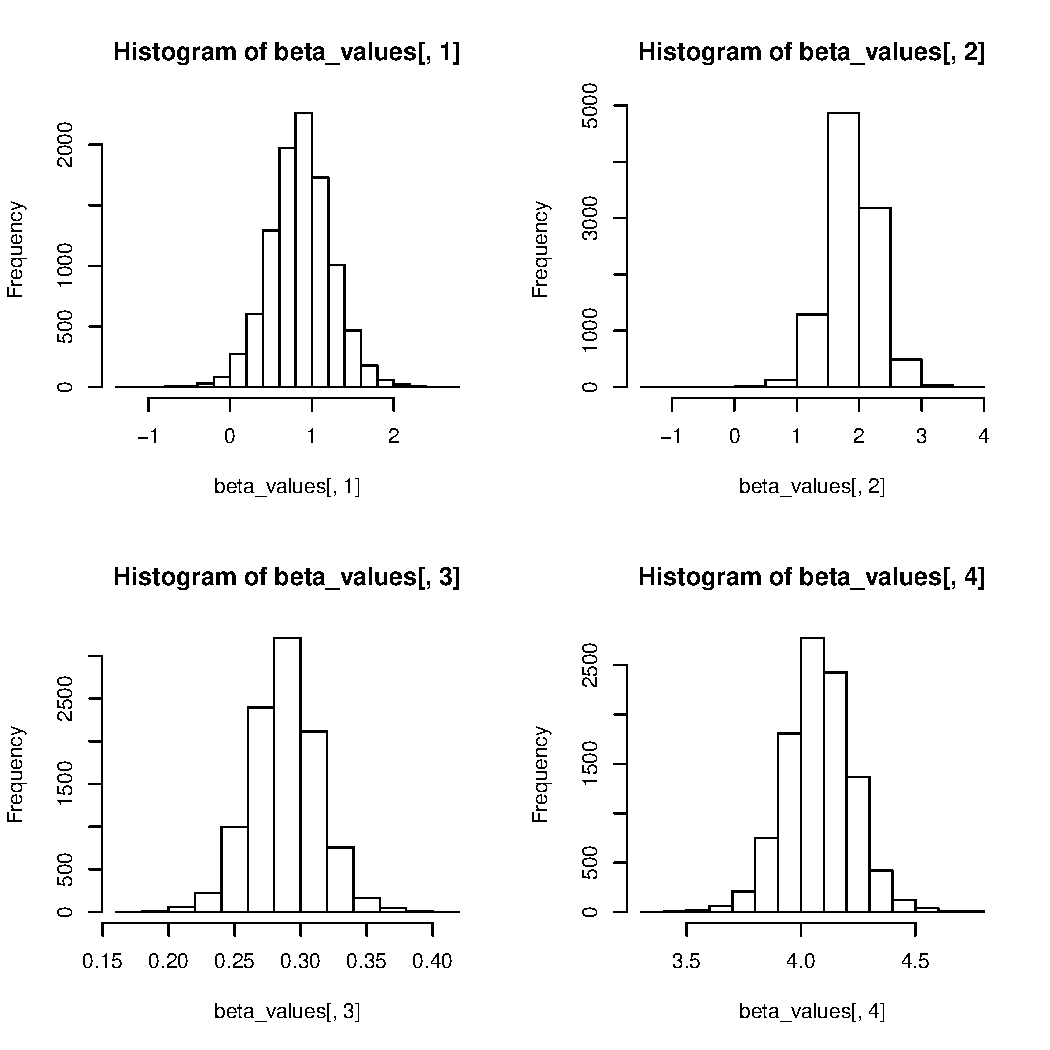
\includegraphics[width=\maxwidth]{figure/unnamed-chunk-7-1} 
\begin{kframe}\begin{alltt}
\hlkwd{par}\hlstd{(}\hlkwc{mfrow}\hlstd{=}\hlkwd{c}\hlstd{(}\hlnum{1}\hlstd{,}\hlnum{1}\hlstd{))}
\end{alltt}
\end{kframe}
\end{knitrout}

\begin{knitrout}
\definecolor{shadecolor}{rgb}{0.969, 0.969, 0.969}\color{fgcolor}\begin{kframe}
\begin{alltt}
\hlcom{## # Bias in c_hat}
\hlkwd{hist}\hlstd{(beta_values[,}\hlnum{4}\hlstd{],} \hlkwc{main} \hlstd{=} \hlstr{"Bootstrapped estimate of c_hat"}\hlstd{)}
\end{alltt}
\end{kframe}
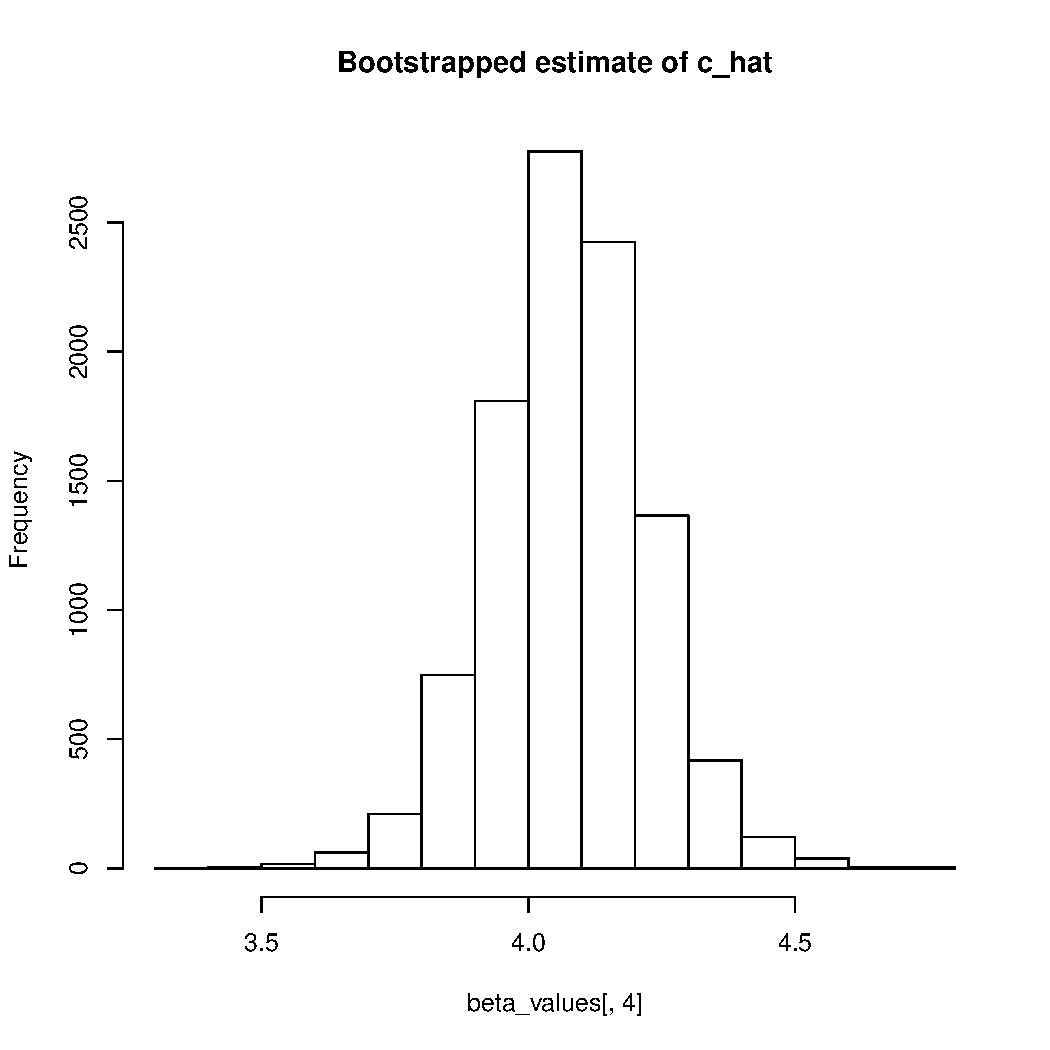
\includegraphics[width=\maxwidth]{figure/unnamed-chunk-8-1} 
\begin{kframe}\begin{alltt}
\hlstd{bias_c} \hlkwb{=} \hlkwd{mean}\hlstd{(beta_values[,}\hlnum{4}\hlstd{])}\hlopt{-}\hlstd{c}
\hlstd{bias_c}
\end{alltt}
\begin{lstlisting}[basicstyle=\ttfamily,breaklines=true]
## [1] 0.07807151
\end{lstlisting}
\end{kframe}
\end{knitrout}

The bias is relatively small when looking at the distribution of c hat. The bootstrapp gives a good estimator of the true parameter. It also gives an accurate confidence interval for the estimate.
\\
If we wanted to evaluate the bias with only one iteration, we would
have obtained:
\begin{knitrout}
\definecolor{shadecolor}{rgb}{0.969, 0.969, 0.969}\color{fgcolor}\begin{kframe}
\begin{alltt}
\hlstd{beta_values_0} \hlkwb{=} \hlkwd{bootstrap_fgls}\hlstd{(}\hlkwc{B}\hlstd{=}\hlnum{1}\hlstd{)}
\hlcom{# bias}
\hlkwd{mean}\hlstd{(beta_values[}\hlnum{4}\hlstd{])}\hlopt{-}\hlstd{c}
\end{alltt}
\begin{lstlisting}[basicstyle=\ttfamily,breaklines=true]
## [1] -2.835923
\end{lstlisting}
\end{kframe}
\end{knitrout}

\end{document}









